\section{Finding Clusters} \label{sect:finding}


\begin{figure*}
    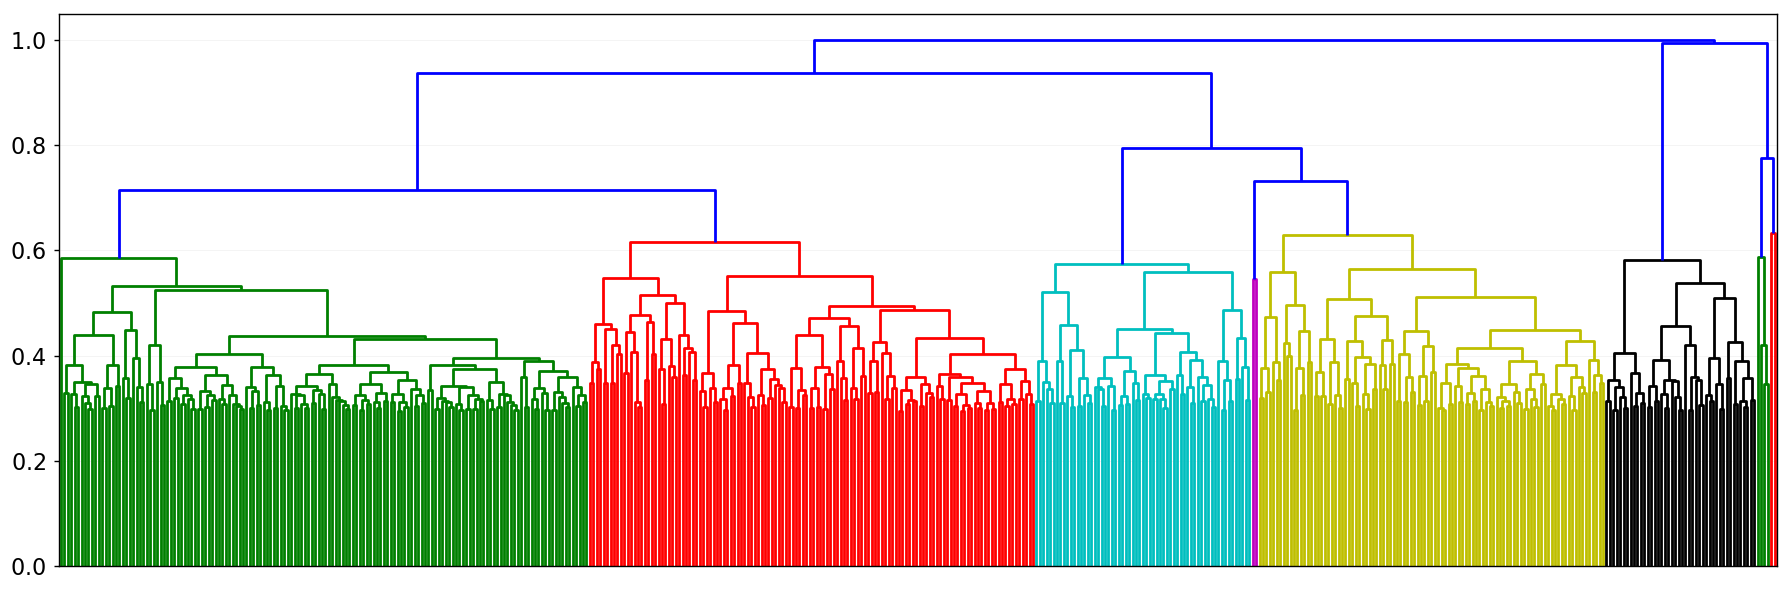
\epsfig{file=figs/dendrograms/v0.png, width=1\linewidth}
    \caption{Dendrogram of CNRE distance across all client pairs}
\end{figure*}


\begin{figure*}
    \center
        \mbox{
            \begin{subfigure}[b]{0.25\linewidth}
                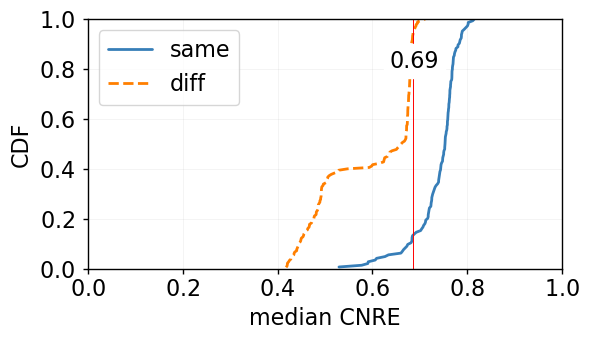
\epsfig{file=figs/cnre_vs_category/country.png, width=1\linewidth}
                \caption{country} 
            \end{subfigure}
            \begin{subfigure}[b]{0.25\linewidth}
                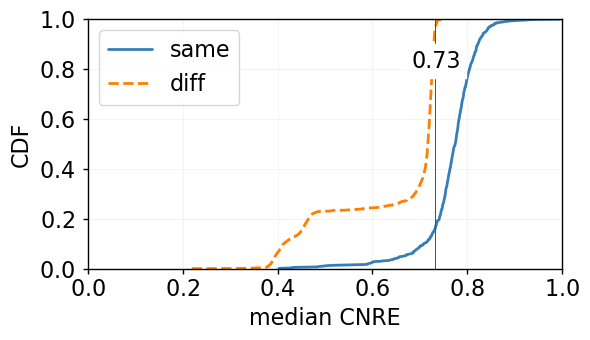
\epsfig{file=figs/cnre_vs_category/asn.png, width=1\linewidth}
                \caption{ASN} 
            \end{subfigure}
            \begin{subfigure}[b]{0.25\linewidth}
                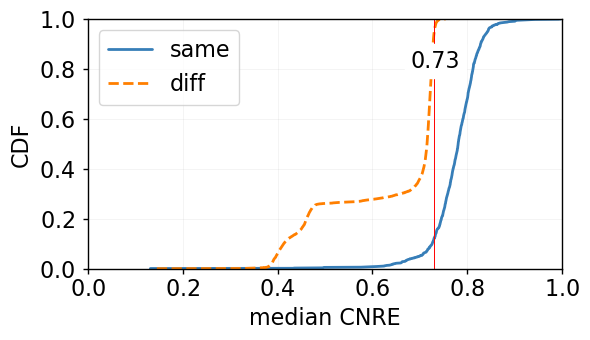
\epsfig{file=figs/cnre_vs_category/prefix.png, width=1\linewidth}
                \caption{BGP prefix} 
            \end{subfigure}
            \begin{subfigure}[b]{0.25\linewidth}
                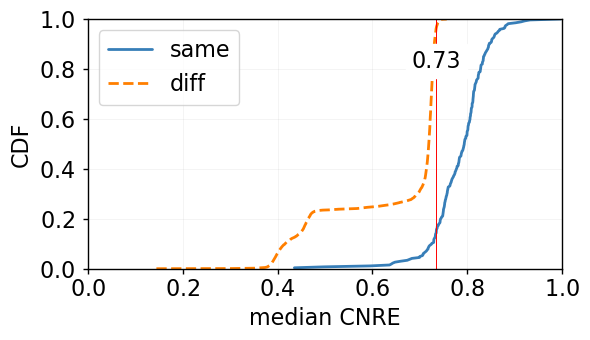
\epsfig{file=figs/cnre_vs_category/ip24.png, width=1\linewidth}
                \caption{IP /24 subnet} 
            \end{subfigure}
        }
    \caption{CDFs of CNREs across client sets with matching (same) and non-matching (diff) labels. 
    ``Same'' shows the CDF for the median CNRE distance across all client pairs matching a given label. 
    ``Diff'' shows the CDF for the median CNRE distance from each label group toward all other labels.}

\end{figure*}


\begin{figure}
    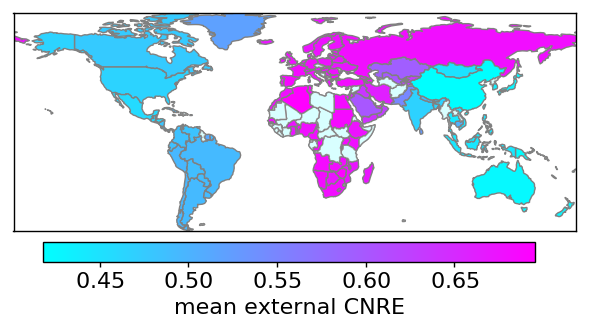
\epsfig{file=figs/cnre_country_uniqueness_map.png, width=1\linewidth}
    \caption{Choropleth with each country shaded by its median CNRE distance from all other countries. TODO: add legend (I'm struggling to format it in geopandas...)}
\end{figure}

\begin{figure*}
    \center
        \mbox{
            \begin{subfigure}[b]{0.25\linewidth}
                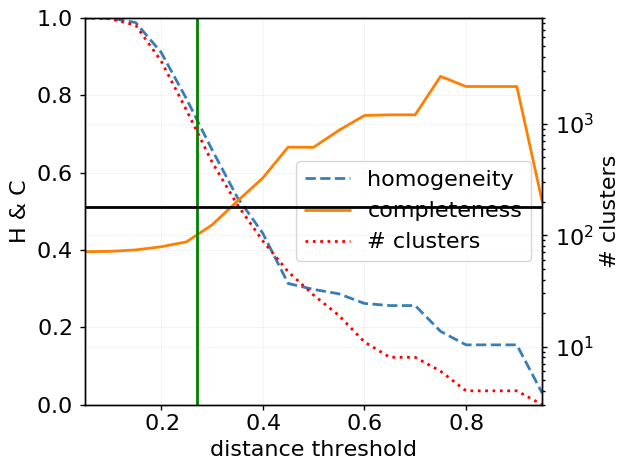
\epsfig{file=figs/completeness_vs_homogeneity/country.png, width=1\linewidth}
                \caption{country} 
            \end{subfigure}
            \begin{subfigure}[b]{0.25\linewidth}
                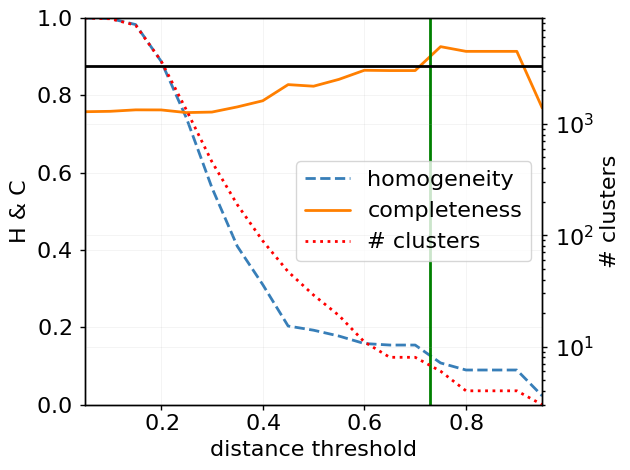
\epsfig{file=figs/completeness_vs_homogeneity/asn.png, width=1\linewidth}
                \caption{ASN} 
            \end{subfigure}
            \begin{subfigure}[b]{0.25\linewidth}
                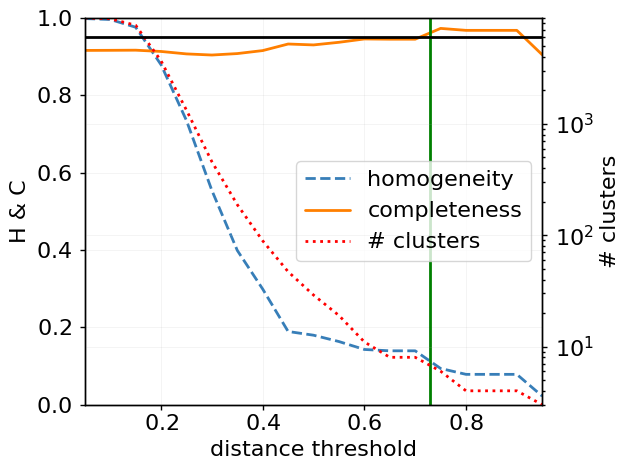
\epsfig{file=figs/completeness_vs_homogeneity/prefix.png, width=1\linewidth}
                \caption{BGP prefix} 
            \end{subfigure}
            \begin{subfigure}[b]{0.25\linewidth}
                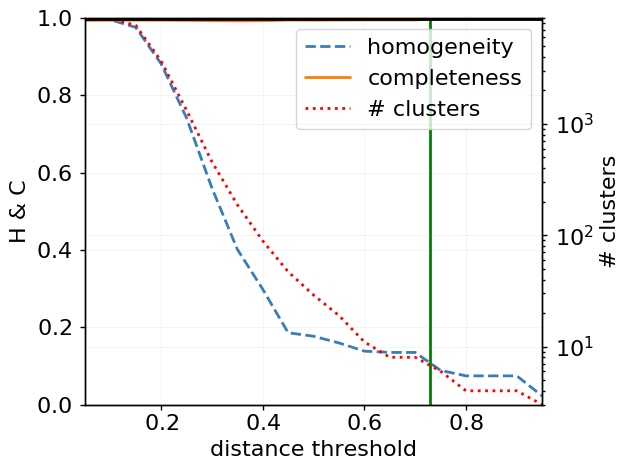
\epsfig{file=figs/completeness_vs_homogeneity/ip24.png, width=1\linewidth}
                \caption{IP /24 subnet} 
            \end{subfigure}
        }
    \caption{Completeness / homogeneity for [country / ASN / bgp prefix / 24 / local resolver] vs clustering distance threshold (this will either be several lines on one plot or an array of subplots)}
\end{figure*}
